\section{Methods} \label{sec:methods} 
\subsection{Hierarchical Bayesian Inference} \label{sec:hier} 
Our goal in this paper is to infer the posterior of cosmological parameters
$\Omega = \{ \Omega_m, \sigma_8 \}$ and baryonic feedback parameters
$\mathcal{B} = \{ A_{\rm SN1}, A_{\rm SN2}, A_{\rm AGN1}, A_{\rm AGN2}\}$ from
the observed photometry of galaxies in the NSA catalog, $\{\bfi X_i\}$:
$p(\Omega, \mathcal{B} \given \{{\bfi X_i}\})$.
${\bfi X_i}$ represents both the measured absolute magnitudes and
uncertainties: $\{ \hat{X}_i, \sigma_{X,i}\}$. 
With our forward model, based on CAMELS-TNG, we can simulate noisy galaxy
photometry from $\Omega$ and $\mathcal{B}$. 
Hence, the cosmological inference from photometry can be reformulated as a
hierarchical population inference problem. 

To illustrate this, we graphically represent our forward model in
Figure~\ref{fig:graph}.
Circles, shaded circles, and dots represent random variables, observed
quantities, and random variables that are deterministic. 
$\theta_i^g$ represents the physical properties of galaxies (\emph{e.g.} $M_*$,
star-formation history), which are determined from $\Omega$ and $\mathcal{B}$
through the CAMELS-TNG simulation.
Then the noisy photometry $\hat{X}_i$ is determined from $\theta_i^g$ through
SPS and our noise model. 

\begin{figure}[ht]
\vskip 0.2in
\begin{center}
    \centerline{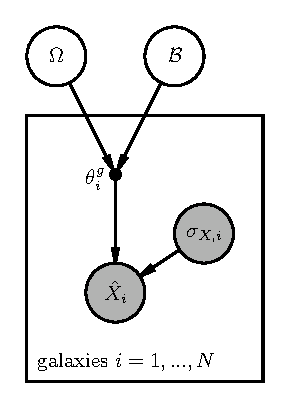
\includegraphics[width=0.6\columnwidth]{figs/graph.pdf}}
    \caption{
        Graphical representation of our hierarchical approach that illustrate
        the relationship among the parameters of our model. 
        Circles are inferred random variables, shaded circles are observed
        quantities, and dots indicate random variables that are deterministic.
        The physical properties of galaxies, $\theta^g_i$, are determined from
        the cosmological and hydrodynamical parameters $\Omega$ and
        $\mathcal{B}$ through the CAMELS-TNG simulation. 
        Then the noisy optical photometry, $\hat{X}_i$, is derived from
        $\theta^g_i$ using SPS and our noise model. 
    }\label{fig:graph}
\end{center}
\vskip -0.2in
\end{figure}

Given this hierarchical model, we can rewrite the posterior as: 
\begin{align}
p(\Omega, \mathcal{B} \given \{{\bfi X_i}\}) 
    =&~\frac{p(\Omega, \mathcal{B})~p(\{{\bfi X_i}\} \given \Omega,
    \mathcal{B})}{p(\{{\bfi X_i}\})}\\
    =&~\frac{p(\Omega, \mathcal{B})}{p(\{\bfi X_i\})}\prod\limits_{i=1}^N 
    p({\bfi X_i}\given \Omega, \mathcal{B})\\
    =&~\frac{p(\Omega, \mathcal{B})}{p(\{\bfi X_i\})}\prod\limits_{i=1}^N 
    \frac{p(\bfi X_i)\,p(\Omega, \mathcal{B}\given{\bfi X_i})}{p(\Omega,
    \mathcal{B})}\\
    %    =&~\frac{p(\Omega, \mathcal{B})}{p(\{{\bfi X_i}\})}\int p(\{{\bfi X_i}\}
    %    \given \{\theta^g_i\})~p(\{\theta^g_i\} \given \Omega, \mathcal{B})~{\rm d}\{\theta^g_i\}.\\
    %    =&~\frac{p(\Omega, \mathcal{B})}{p(\{{\bfi X_i}\})}\prod\limits_{i=1}^N\int
    %    p({\bfi X_i} \given \theta^g_i)~p(\theta^g_i \given \Omega, \mathcal{B})~{\rm d}\theta^g_i\\
    %    =&~\frac{p(\Omega, \mathcal{B})}{p(\{{\bfi X_i}\})}\prod\limits_{i=1}^N\int
    %    \frac{p(\theta^g_i \given {\bfi X_i})~p({\bfi
    %    X_i})}{p(\theta^g_i)}~p(\theta^g_i \given \Omega, \mathcal{B})~{\rm d}\theta^g_i\\
    %    =&~p(\Omega, \mathcal{B})\prod\limits_{i=1}^N\int \frac{~p(\theta^g_i
    %    \given \Omega, \mathcal{B})}{p(\theta^g_i)} p(\theta^g_i \given {\bfi X_i})
    %    ~{\rm d}\theta^g_i\\
    %    =&~p(\Omega, \mathcal{B})\prod\limits_{i=1}^N\int \frac{p(\Omega, \mathcal{B}\given \theta^g_i)}{p(\Omega, \mathcal{B})}
    %p(\theta^g_i \given {\bfi X_i})~{\rm d}\theta^g_i \\
    %     \label{eq:post0}
    %    =&~\frac{1}{p(\Omega, \mathcal{B})^{N-1}}\prod\limits_{i=1}^N\int p(\Omega,
    %    \mathcal{B}\given \theta^g_i) p(\theta^g_i \given {\bfi X_i})~{\rm
    %    d}\theta^g_i  \\
    %     \label{eq:posterior}
    =&~\frac{1}{p(\Omega, \mathcal{B})^{N-1}}\prod\limits_{i=1}^N p(\Omega,
    \mathcal{B}\given {\bfi X_i})\\
\intertext{
    We downsampled the galaxies in the CAMELS-TNG simulations to impose 
    $p(\Omega, \mathcal{B}) = 1$ (Sec.~\ref{sec:sims}), so the posterior
    simply becomes:}
    \label{eq:posterior}
    =&~\prod\limits_{i=1}^N p(\Omega, \mathcal{B}\given {\bfi X_i}).
\end{align} 
Hence, we can evaluate $p(\Omega, \mathcal{B} \given \{{\bfi X_i}\})$, and
sample it, as long as we can accurately estimate $p(\Omega, \mathcal{B}\given
{\bfi X_i})$, the posterior for photometry from an individual galaxy. 

\subsection{Neural Density Estimation} \label{sec:anpe}
One way to accurately estimate $p(\Omega, \mathcal{B}\given {\bfi X_i})$ is
by applying neural density estimation (NDE) to the CAMELS-TNG.
The CAMELS-TNG forward model provides a training dataset of 100,000
parameter-photometry pairs: $\{(\Omega, \mathcal{B}, {\bfi X_i})\}$.
With NDE, we can use this data to train a neural network $q$ with parameters
$\phi$ to estimate 
$p(\Omega, \mathcal{B}\given {\bfi X_i}) \approx
q_\phi(\Omega, \mathcal{B}\given {\bfi X_i})$.
This type of simulaiton-based inference using NDE has now been applied to a
broad range of astronomical applications:
\eg~analyzing gravitational waves~\citep{wong2020, dax2021}, binary
microlensing lensing~\citep{zhang2021}, galaxy SEDs~\cite{hahn2022a}, and
galaxy clustering~\cite{hahn2022d, hahn2023}. 

In this work, our NDE is based on ``normalizing flow'' models~\citep{tabak2010,
tabak2013}, which use neural networks to learn a flexible and bijective
transformation, $f$, that maps a complex target distribution to a simple base
distribution that is fast to evaluate.
$f$ is defined to be invertible and have a tractable Jacobian so that the 
target distribution can be evaluated with change of variables. 
Since $\pi(\bfi{z})$ is easy to evaluate, this enables us to also easily 
evaluate the target distribution.
In our case, the target distribution is 
$p(\Omega, \mathcal{B}\given {\bfi X_i})$ and we set the base distribution to
be a multivariate Gaussian. 
Among different flow architectures, we use Masked Autoregressive
Flow~\citep[MAF;][]{papamakarios2017} models implemented in the $\mathtt{sbi}$
Python
package\footnote{\url{https://github.com/mackelab/sbi/}}~\citep{greenberg2019,
tejero-cantero2020}.

\begin{figure}[ht]
\vskip 0.2in
\begin{center}
    \centerline{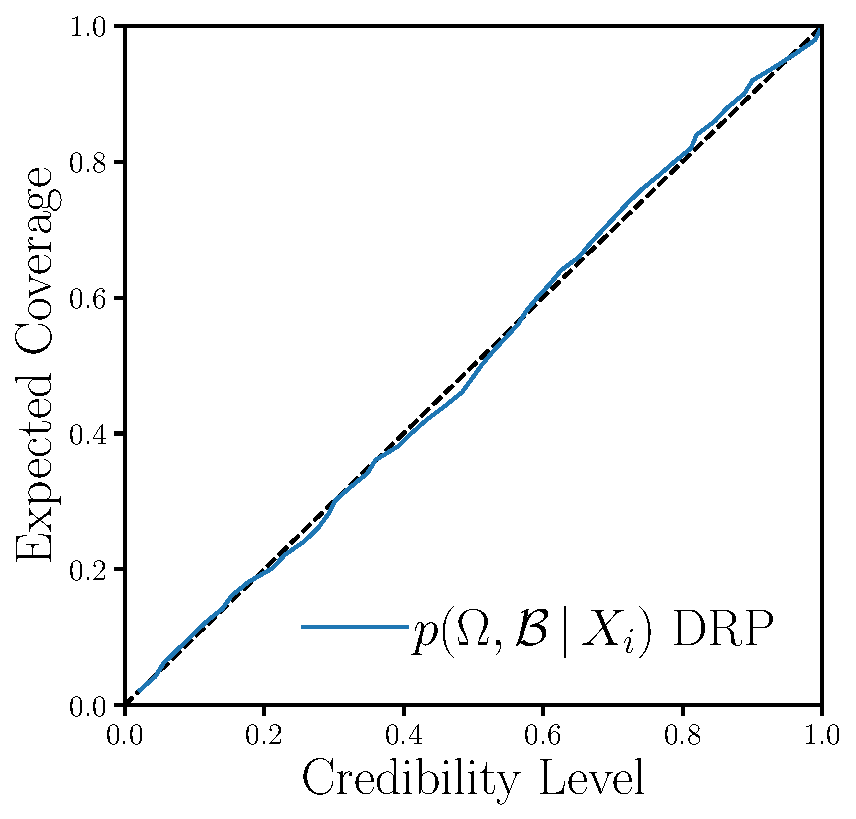
\includegraphics[width=0.6\columnwidth]{figs/tarp_p_omega_x.pdf}}
    \caption{DRP coverage test validating the accuracy of our 
    $q_{\phi}(\Omega, \mathcal{B}\given {\bfi X_i})$ posterior estimate trained
    using the forward modeled CAMELS-TNG data (blue).
    The black-dashed line represents an optimal estimate of the posterior.
    The coverage test demonstrates that $q_\phi$ provides a near optimal
    estimate of the true posterior.
    }\label{fig:tarp}
\end{center}
\vskip -0.2in
\end{figure}

Our goal in training the flow is to determine $q_\phi$ that best approximates 
$p(\Omega, \mathcal{B}\given {\bfi X_i})$. 
We can reformulate this into an optimization problem for determining $\phi$
that minimizes the KL divergence between 
$p(\Omega, \mathcal{B}, {\bfi X_i}) = p(\Omega, \mathcal{B}\given {\bfi X_i})
 p({\bfi X_i})$ and
$q_\phi(\Omega, \mathcal{B}\given {\bfi X_i}) p({\bfi X_i})$.
In practice, we split the $\{(\Omega, \mathcal{B}, {\bfi X_i}\}$ data from
CAMELS-TNG into a training and validation set with a 90/10 split.
Then, we maximize the total log-likelihood 
$\sum_i \log q_{\phi}(\Omega, \mathcal{B}\given {\bfi X_i})$ over the 
training set, which is equivalent to the KL divergence, using the {\sc Adam} 
optimizer~\citep{kingma2017} with a learning rate of $5\times10^{-4}$. 
To prevent overfitting, we evaluate the total log-likelihood on the validation
data at every training epoch and stop the training when the validation 
log-likelihood fails to increase after 20 epochs.  


We determine the architecture of our flow by training a large number of flows
with architectures determined using the \cite{akiba2019} hyperparameter optimization framework.
Afterwards, we define our final flow as an equally weighted ensemble of five
flows with the lowest validation losses: 
$q_{\phi}(\Omega, \mathcal{B}\given {\bfi X_i}) = 
\sum_{j=1}^5 q_{\phi,j}(\Omega, \mathcal{B}\given {\bfi X_i})/5$. 
Ensembling flows with different initializations and architectures improves the
overall robustness of our normalizing flow~\citep{alsing2019}.
To validate the accuracy of $q_\phi$, we use the ``distance to random point''
(DRP) coverage test from \cite{lemos2023}, which is necessary and sufficient to
show that a posterior estimator is optimal. 
In Fig~\ref{fig:tarp}, we present the DRP coverage of $q_\phi$ (blue) and
find that it provides a near optimal estimate of the true posterior.


\begin{figure}[ht]
\vskip 0.2in
\begin{center}
    \centerline{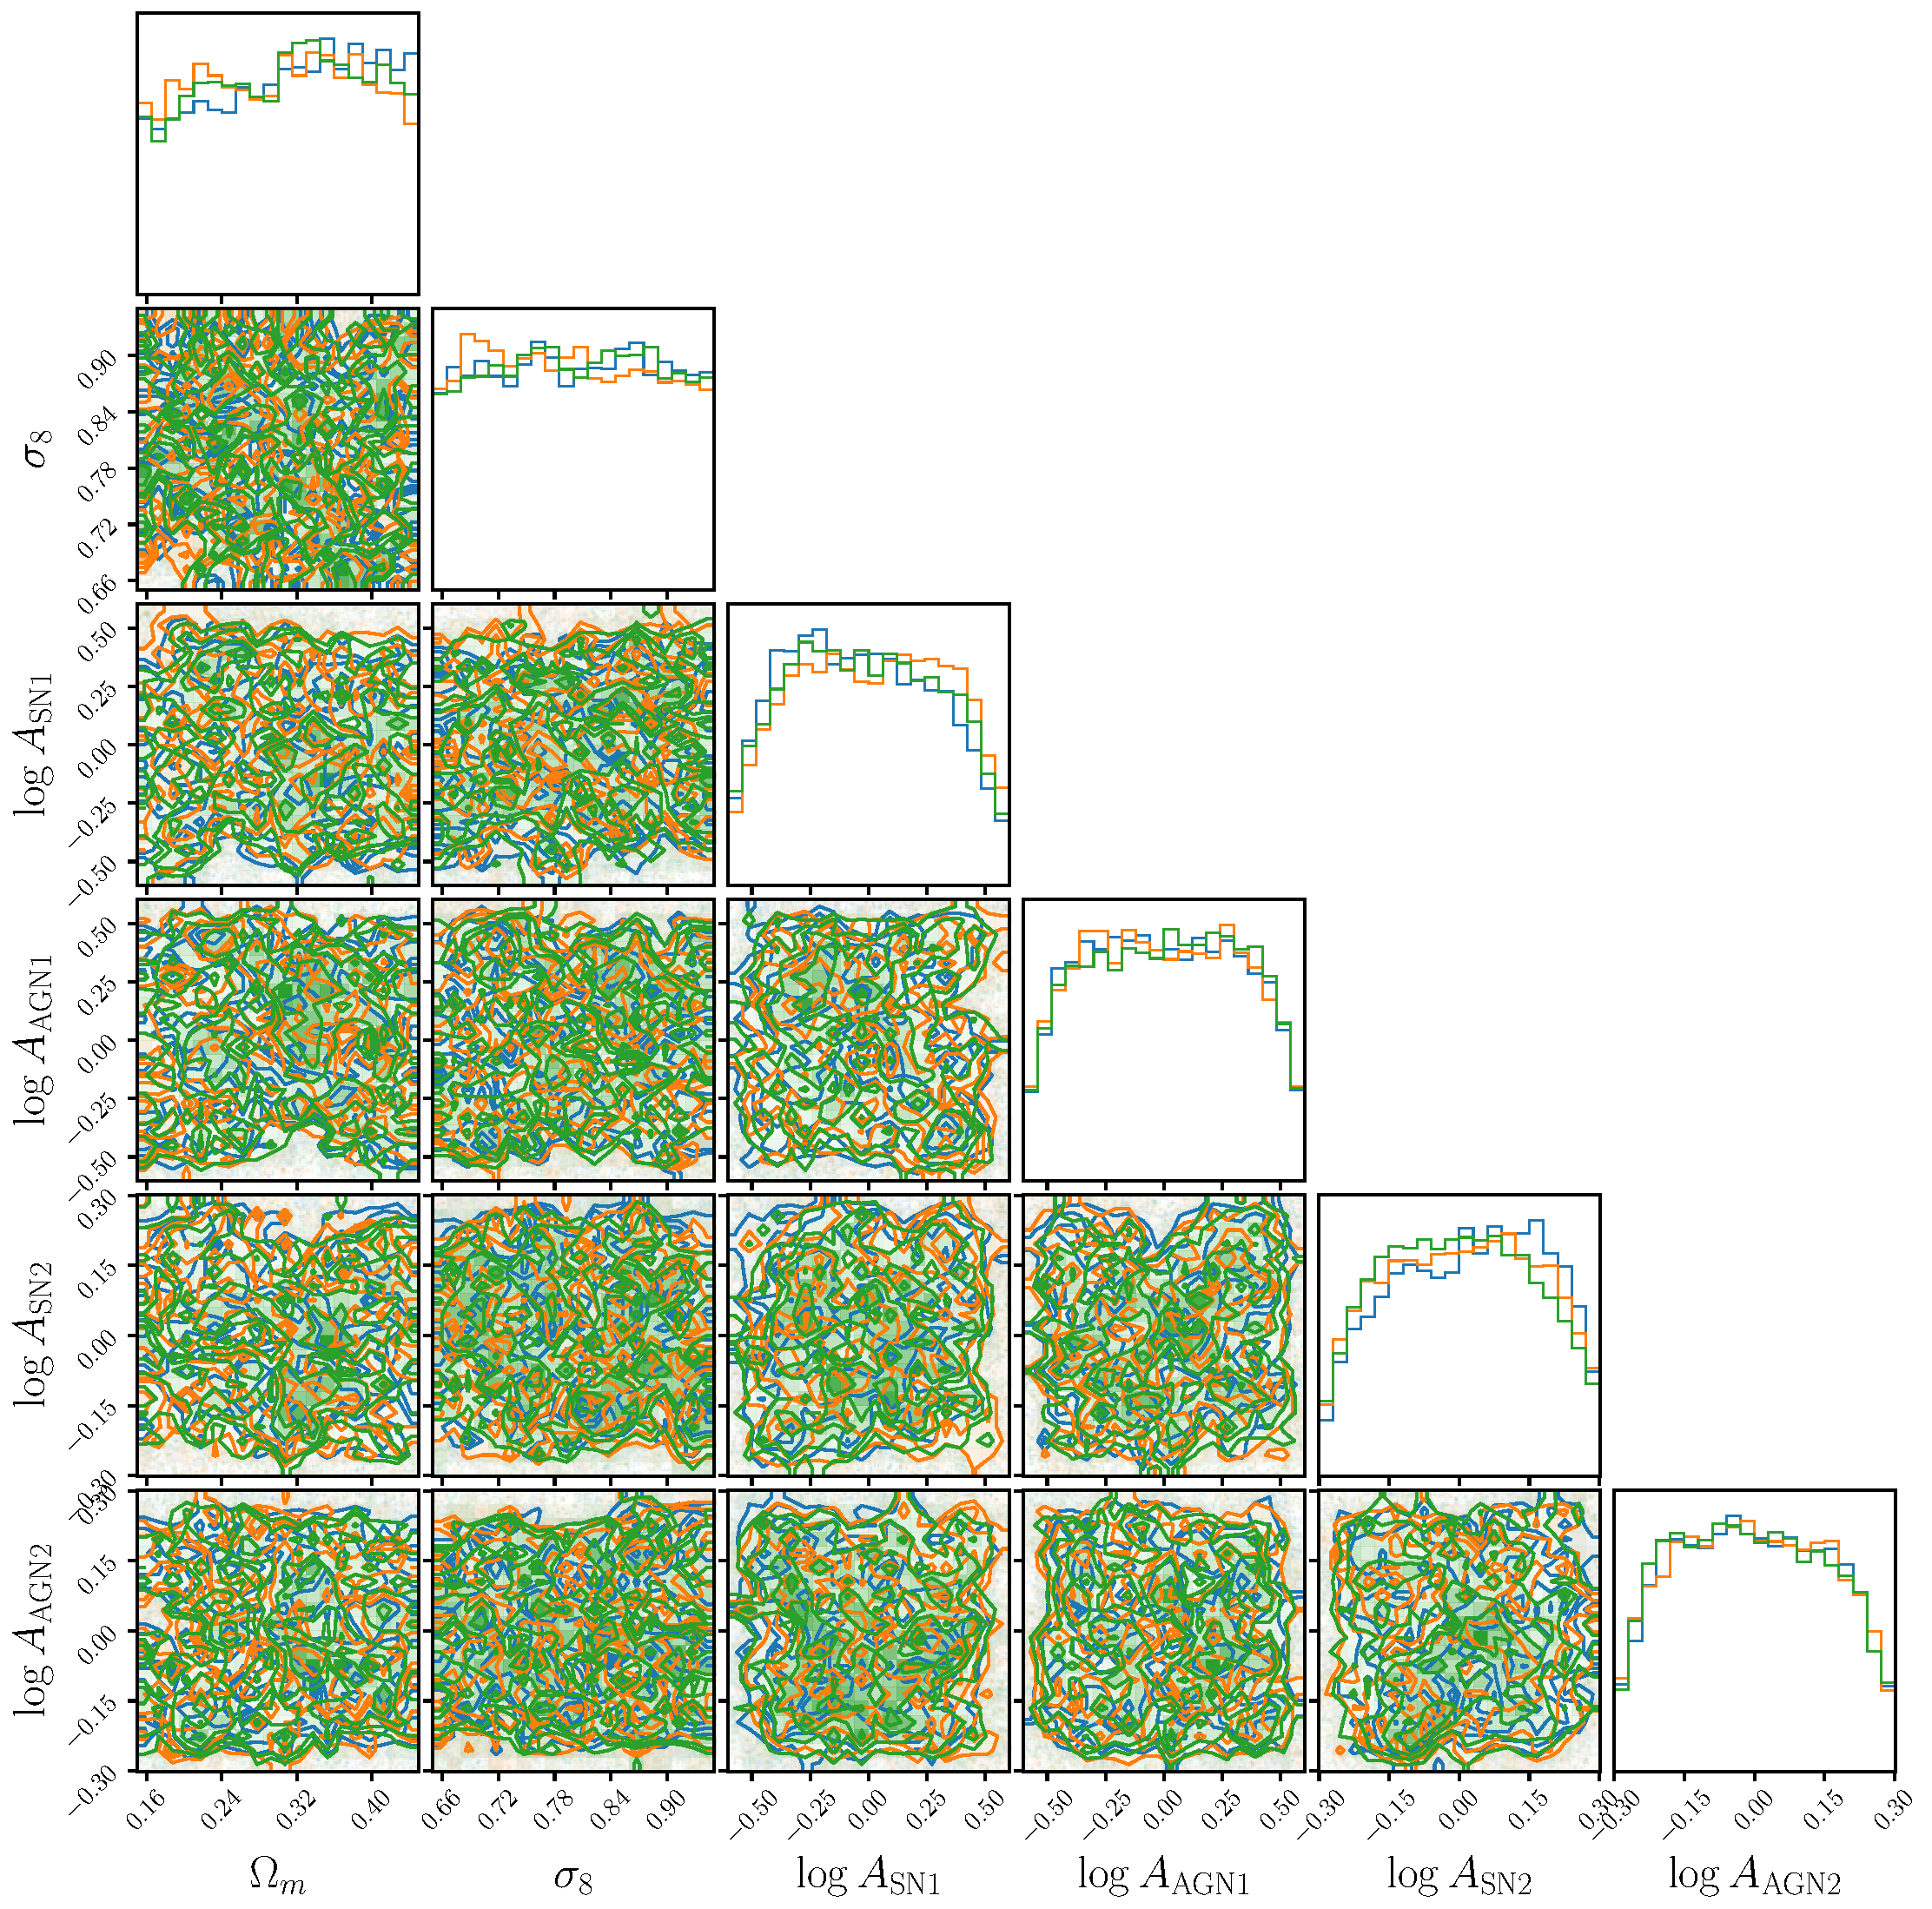
\includegraphics[width=\columnwidth]{figs/p_omega_x_i.pdf}}
    \caption{Estimated posteriors of the cosmological and hydrodynamical 
    parameters ($\Omega$, $mathcal{B}$) from photometry, 
    $q_{\phi}(\Omega, \mathcal{B}\given {\bfi X_i})$,for three arbitrarily 
    selected NSA galaxies. 
    The posteriors correspond to the galaxies marked in Fig.~\ref{fig:nsa}.
    }\label{fig:p_omega_x_i}
\end{center}
\vskip -0.2in
\end{figure}

In Fig.~\ref{fig:p_omega_x_i}, we present 
$q_{\phi}(\Omega, \mathcal{B}\given {\bfi X_i})$
for three arbitrarily selected NSA galaxies. 
The selected galaxies are also marked in Fig.~\ref{fig:nsa}. 
The individual posteriors reveal that  there is very little cosmological
information in the photometry of a single galaxy. 
However, with Eq.~\ref{eq:posterior}, we can extract the cosmological
information from {\em thousands} of galaxies.
